\documentclass[a4paper,10pt,dvipdfmx]{jsarticle}

\usepackage[dvipdfmx]{graphicx}
\usepackage{subcaption}
\usepackage{url}
\usepackage{bm}
\usepackage{amsmath,amssymb}
\usepackage{ascmac}

%\captionsetup[subfigure]{labelformat=simple}
\renewcommand{\thesubfigure}{(\alph{subfigure})}

\newcommand{\qed}{\hfill$\Box$}
\newcommand{\Proof}{\noindent{\bf Proof.}\quad}
\makeatletter
\newcommand{\figcaption}[1]{\def\@captype{figure}\caption{#1}}
\newcommand{\tblcaption}[1]{\def\@captype{table}\caption{#1}}
\makeatother

\newcommand{\bhline}[1]{\noalign{\hrule height #1}}  
\newcommand{\bvline}[1]{\vrule width #1}  

\begin{document}

\title{\vspace{-2cm}$\S1.12$ 回帰式による予測値の区間推定(重回帰の場合)\\ $\S1.13$説明変数の選択}
\author{富島諒}
\date{2021年6月17日}

\maketitle

$\S1.11$で紹介した数式は式番号の前に$\clubsuit$を付ける. 

\section{$\S1.12$ 回帰式による予測値の区間推定(重回帰の場合)}
本節の目的は, 
\begin{enumerate}
  \item 重回帰モデルによる目的変数の基本統計量を求める
  \item 基本統計量を元に信頼区間を算出し, 区間推定を行う
\end{enumerate}
である. 

説明変数$(x_1, \cdots, x_p)$がある特定の値$(x_{10}, \cdots, x_{p0})$をとるときの目的変数$y$の期待値$\eta_0$は, 回帰式を用いて
\begin{align}
  \label{eq:model}
  Y_0 = \hat{a}_0 + \hat{a}_1x_{10} + \cdots +\hat{a}_px_{p0}
\end{align}
によって, 推定(予測)することができる. このとき, $Y_0$の期待値は
\begin{align}
  \notag
  \operatorname{E}(Y_0) 
  &= \operatorname{E}(\hat{a}_0 + \hat{a}_1x_{10} + \cdots +\hat{a}_px_{p0})\\
  \notag
  &=\operatorname{E}(\hat{a}_0) + \operatorname{E}(\hat{a}_1)x_{10} + \cdots +\operatorname{E}(\hat{a}_p)x_{p0}\\
  \label{eq:eta_0}
  &=a_0 + a_1x_{10} + \cdots + a_px_{p0} = \eta_0 \\
  \notag
  & \text{\quad ($\because$ $\clubsuit$式(11a)
  \;$\operatorname{E}(\hat{a}_j)=a_j,$
  式(11d)
  \;$\operatorname{E}(\hat{a}_0)=a_0$より)}
\end{align}
となり, 予測値$Y_0$は$\eta_0$に対する不偏推定値である. また$Y_0$の分散は式\eqref{eq:v_y0}のようになる. 

\begin{align}
  \notag %1
  \operatorname{V}(Y_0)
  &= \operatorname{E}\left[
    \left\{
      Y_0-\operatorname{E}(Y_0)
    \right\}^2
  \right]\\
  \notag %2
  &= \operatorname{E}\left[
    \left\{
      (\hat{a}_0 + \hat{a}_1x_{10} + \cdots +\hat{a}_px_{p0}) -(a_0 + a_1x_{10} + \cdots + a_px_{p0})
    \right\}^2
  \right] \\
  \notag
  & \text{\quad ($\because$ 式\eqref{eq:model} \;$Y_0 = \hat{a}_0 + \hat{a}_1x_{10} + \cdots +\hat{a}_px_{p0}$より)} \\
  \notag %3
  &=\operatorname{E}\left[
    \left\{
      \left(
        \hat{a}_0 + \sum_{j=1}^p \hat{a}_jx_{j0}
      \right) -
      \left(
        a_0 + \sum_{j=1}^p a_jx_{j0}
      \right)
    \right\}^2
  \right] \\
  \notag %4
  &= \operatorname{E}\left[
    \left\{
      (\hat{a}_0-a_0)+\sum_{j=1}^px_{j0}(\hat{a}_j-a_j)
    \right\}^2
  \right] \\
  \notag %5
  &= \operatorname{E}\left[
    (\hat{a}_0-a_0)^2 + 2\sum_{j=1}^px_{j0}(\hat{a}_0-a_0)(\hat{a}_j-a_j)
    + \sum_{j=1}^p\sum_{l=1}^px_{j0}x_{l0}(\hat{a}_j-a_j)(\hat{a}_l-a_l)
  \right]\\
  \notag %6
  &= \operatorname{E}\left[
    (\hat{a}_0-a_0)^2
  \right]
  +2\sum_{j=1}^px_{j0}\operatorname{E}\left[
    (\hat{a}_0-a_0)(\hat{a}_j-a_j)
  \right]
  + \sum_{j=1}^p\sum_{l=1}^px_{j0}x_{l0}\operatorname{E}\left[
    (\hat{a}_j-a_j)(\hat{a}_l-a_l)
  \right] \\
  \notag %7
  &= \operatorname{V}(\hat{a}_0) 
  +2\sum_{j=1}^px_{j0}\operatorname{Cov}(\hat{a}_0, \hat{a}_j)
  + \sum_{j=1}^p\sum_{l=1}^px_{j0}x_{l0}\operatorname{Cov}(\hat{a}_j, \hat{a}_l) \\ %8
  \notag
  &= \left(\frac{1}{n}+\sum_{j=1}^p\sum_{l=1}^p\frac{\bar{x}_j\bar{x}_ls^{jl}}{n}\right)\sigma^2
  +2\sum_{j=1}^px_{j0}\left(
    -\sum_{l=1}^p\frac{\bar{x}_ls^{jl}\sigma^2}{n}
  \right)
  + \sum_{j=1}^p\sum_{l=1}^px_{j0}x_{l0}\frac{s^{jl}\sigma^2}{n} \\
  \notag
  \begin{split}
    & \text{\quad ($\because$ $\clubsuit$式(11c)
     \;$\operatorname{Cov}(\hat{a}_j, \hat{a}_l) =\frac{s^{jl}\sigma^2}{n}$, $\clubsuit$式(11e) 
     \; $\operatorname{V}(\hat{a}_0) = \left(\frac{1}{n}+\sum_{j=1}^p\sum_{l=1}^p\frac{\bar{x}_j\bar{x}_ls^{jl}}{n}\right)\sigma^2$} \\
    & \text{\quad $\clubsuit$式(11f) 
    \; $\operatorname{Cov}(\hat{a}_0, \hat{a}_j) = -\sum_{l=1}^p\frac{\bar{x}_ls^{jl}\sigma^2}{n}$)}
  \end{split} \\
  \notag %9
  &= \left\{
    \frac{1}{n} + \frac{1}{n}\left(
      \sum_{j=1}^p\sum_{l=1}^p\bar{x}_j\bar{x}_ls^{jl}
      -2\sum_{j=1}^p\sum_{l=1}^px_{j0}\bar{x}_ls^{jl}
      + \sum_{j=1}^p\sum_{l=1}^px_{j0}x_{l0}s^{jl}
    \right)
  \right\}\sigma^2 \\
  \notag
  &= \left\{
    \frac{1}{n} + \frac{1}{n}\sum_{j=1}^p\sum_{l=1}^p(\bar{x}_j\bar{x}_l-x_{j0}\bar{x}_l-x_{l0}\bar{x}_j+x_{j0}x_{l0})s^{jl}
  \right\}\sigma^2 \\
  \label{eq:v_y0} %10
  &= \left\{
    \frac{1}{n} + \frac{1}{n}\sum_{j=1}^p\sum_{l=1}^p(x_{j0}-\bar{x}_j)(x_{l0}-\bar{x}_l)s^{jl}
  \right\}\sigma^2
\end{align}

ここで$Y_0$を標準化すると, 
\begin{align*}
  u 
  &= \frac{Y_0-\operatorname{E}(Y_0)}{\sqrt{\operatorname{V}(Y_0)}} \\
  &= \frac{Y_0-\eta_0}{\sqrt{\left\{
    \frac{1}{n} + \frac{1}{n}\sum_{j=1}^p\sum_{l=1}^p(x_{j0}-\bar{x}_j)(x_{l0}-\bar{x}_l)s^{jl}
  \right\}\sigma^2}}
\end{align*}
となる. $u$は標準正規分布$N(0, 1)$に従う. ただし, このとき未知の誤差分散$\sigma^2$を含んでおり, これを不偏推定値$\operatorname{V}_e=\frac{\operatorname{F}_(\hat{a}_0, \hat{a}_1, \cdots, \hat{a}_p)}{n-p-1}$で置き換えて得られる統計量は, 
\begin{align}
  \label{eq:stat_unbiased_estimate}
  t = \frac{Y_0-\eta_0}{\sqrt{\left\{
    \frac{1}{n} + \frac{1}{n}\sum_{j=1}^p\sum_{l=1}^p(x_{j0}-\bar{x}_j)(x_{l0}-\bar{x}_l)s^{jl}
  \right\}\operatorname{V}_e}}
\end{align}
となる. 

ここで, 
\begin{align}
  \label{eq:eq:Mahalanobis}
  \operatorname{D}_0^2
  = \sum_{j=1}^p\sum_{l=1}^p(x_{j0}-\bar{x}_j)(x_{l0}-\bar{x}_l)s^{jl}
\end{align}
とする. この$\operatorname{D}_0^2$は単回帰における, 
\begin{align}
  \label{eq:single_regre}
  t= 
  \frac{Y_0-\eta_0}
  {\sqrt{
    \left\{
      \frac{1}{n}+\frac{(x_0-\bar{x})^2}{ns_{xx}}
    \right\}\operatorname{V}_e
  }}
\end{align}
式\eqref{eq:single_regre}の分母の$(x_0-\bar{x})^2/s_{xx}$(=標準偏差で標準化した平均からの距離の2乗)を重回帰の場合に一般化したものに相当し, 点$(x_{10}, \cdots, x_{p0})$と重心$(\bar{x}_1, \cdots, \bar{x}_p)$との間の{\bf マハラノビスの汎距離}\footnote{\url{https://www.sist.ac.jp/~kanakubo/research/statistic/hanbetu_maha.html}}と呼ばれる. 

\begin{itembox}[l]{マハラノビスの汎距離}
  \quad 図の緑の点を赤色の点のグループか青色の点のグループに属するかを考える. このとき, 赤色のグループの平均点と青色のグループの平均点に関してユークリッド距離で比較すると, 赤色のグループの方が近いのでに緑色の点は赤色の区分される. しかし, 緑は青色に挟まれているので青色のグループに区分されるのが妥当だと考えられる. このように全てのデータの分布に応じた距離を定義するもののひとつがマハラノビス汎距離である.
\end{itembox}

\begin{figure}[htb]
  \centering
  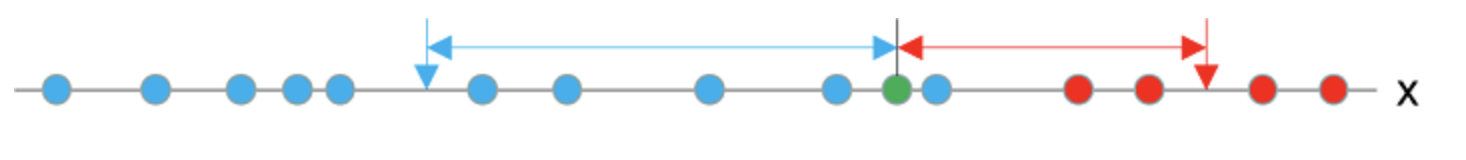
\includegraphics[width=14cm]{../pics/mahara.png}
  \caption{マハラノビスの汎距離}
  \label{fig:mahalanobis}
\end{figure}

式\eqref{eq:eq:Mahalanobis}を用いると, 式\eqref{eq:stat_unbiased_estimate}は次のようになる. 
\begin{align}
  \label{eq:stat_ve}
  t
  = \frac{Y_0-\eta_0}
  {\sqrt{\left\{
    \frac{1}{n} + \frac{1}{n}\operatorname{D}_0^2
  \right\}\operatorname{V}_e}}
\end{align}
このとき, $t$は自由度$n-p-1$のt分布に従い, $\eta_0$に対する信頼率$1-\alpha$の信頼区間は, 
\begin{align*}
  -t_{\alpha}(n-p-1) \leq
  \frac{Y_0-\eta_0}
  {\sqrt{\left(
    \frac{1}{n} + \frac{1}{n}\operatorname{D}_0^2
  \right)\operatorname{V}_e}}
  \leq t_{\alpha}(n-p-1)
\end{align*}
すなわち, 
\begin{align}
  \label{eq:confidence_interval}
  Y_0-t_{\alpha}(n-p-1)\sqrt{\left\{
    \frac{1}{n} + \frac{1}{n}\operatorname{D}_0^2
  \right\}}\operatorname{V}_e 
  \leq \eta_0
  \leq Y_0 + t_{\alpha}(n-p-1)\sqrt{\left\{
    \frac{1}{n} + \frac{1}{n}\operatorname{D}_0^2
  \right\}}\operatorname{V}_e 
\end{align}
のようになる. 式\eqref{eq:confidence_interval}で, $\operatorname{D}_0^2$の小さいところ, すなわち重心の近くでは信頼区間の巾が小さく, $\operatorname{D}_0^2$の大きいところ, すなわち重心から遠く離れたところでは信頼区間の巾が大きくなることがわかる.  \\

次に, 説明変数の特定の値$(x_{10}, \cdots, x_{p0})$に対応して得られるであろう目的変数$y$の値の信頼区間について考える. $y$は今までに観測されている$(y_1, \cdots, y_n)$やそれらに基づく$\hat{a}_1, \cdots, \hat{a}_p$とは独立に平均$\eta_0$, 分散$\sigma^2$の正規分布に従うため, $Y_0-y$の期待値と分散は, 
\begin{align}
  \notag
  \operatorname{E}(Y_0-y)
  &= \operatorname{E}(Y_0) - \operatorname{E}(y)\\
  \notag
  &= \eta_0 -\eta_0 \text{\quad ($\because$ 式\eqref{eq:eta_0} \;$\operatorname{E}(Y_0)=\eta_0$より)} \\
  \label{eq:E_y0-y}
  &= 0 \\
  \notag
  \\
  \notag
  \operatorname{V}(Y_0-y)
  &= \operatorname{E}\left[
    (Y_0-y)^2
  \right] \\
  \notag
  &= \operatorname{E}\left[
    \left\{
      (Y_0-\eta_0) - (y-\eta_0)
    \right\}^2
  \right] \\
  \notag
  &= \operatorname{E}\left[
    (Y_0-\eta_0)^2
  \right]
  +\operatorname{E}\left[
    (y-\eta_0)^2
  \right]
  -2\operatorname{E}\left[
    (Y_0-\eta_0)(y-\eta_0)
  \right] \\
  \notag
  &= \operatorname{V}(Y_0) + \operatorname{V}(y)-2\operatorname{Cov}(Y_0, y) \\
  \notag
  &=\operatorname{V}(Y_0) + \operatorname{V}(y) \text{\quad ($\because$ \;$Y_0$と$y$は無相関)} \\
  \notag
  &= \left(
    \frac{1}{n} + \frac{1}{n}\operatorname{D}_0^2
  \right)\sigma^2 
  + \sigma^2 \\
  \notag
  &\text{\quad ($\because$ 式\eqref{eq:v_y0} \;$\operatorname{V}(Y_0)=\left\{
    \frac{1}{n} + \frac{1}{n}\sum_{j=1}^p\sum_{l=1}^p(x_{j0}-\bar{x}_j)(x_{l0}-\bar{x}_l)s^{jl}
  \right\}\sigma^2$より)} \\
  \label{eq:V_y0-y}
  &= \left(
    1+\frac{1}{n} + \frac{1}{n}\operatorname{D}_0^2
  \right)\sigma^2
\end{align}
となる. これを用いて, $Y_0-y$を標準化し, $\sigma^2$を不偏推定値$\operatorname{V}_e=\frac{\operatorname{F}(\hat{a}_0, \hat{a}_1, \cdots, \hat{a}_p)}{n-p-1}$で置き換えると, 式\eqref{eq:t'}を得る. $t'$は自由度$n-p-1$のt分布に従う. 
\begin{align}
  \label{eq:t'}
  t'
  = \frac{Y_0-y}{\sqrt{\left(
    1+\frac{1}{n} + \frac{1}{n}\operatorname{D}_0^2
  \right)\operatorname{V}_e}}
\end{align}
これより, $(x_{10}, \cdots, x_{p0})$に対応して観測される目的変数$y$に対する信頼率$1-\alpha$の信頼区間は, 
\begin{align*}
  -t_\alpha(n-p-1) 
  \leq \frac{Y_0-y}{\sqrt{\left(
    1+\frac{1}{n} + \frac{1}{n}\operatorname{D}_0^2
  \right)\operatorname{V}_e}}
  \leq t_\alpha(n-p-1) 
\end{align*}
すなわち, 
\begin{align}
  \label{eq:confidence_interval_Y0}
  Y_0-t_{\alpha}(n-p-1)\sqrt{\left(
    1+\frac{1}{n} + \frac{1}{n}\operatorname{D}_0^2
  \right)\operatorname{V}_e}
  \leq y \leq
  Y_0+t_{\alpha}(n-p-1)\sqrt{\left(
    1+\frac{1}{n} + \frac{1}{n}\operatorname{D}_0^2
  \right)\operatorname{V}_e}
\end{align}
のように与えられる. 

\section{$\S1.13$説明変数の選択}
これまでの議論では,回帰モデルに含まれる説明変数$x_{1}, \cdots, x_{p}$は定められたものとして回帰係数や予測値を計算してきた. しかし, 実際に現象を分析する場合には, 目的変数$y$に影響を及ぼすかもしれないと考えられる変数は多数あり, その中から次のようなことを考慮し, しかも実質科学的にも重要な変数を取り上げるのが普通である. 

\begin{enumerate}
  \item 回帰モデルに無駄な変数(真の回帰係数が0であるような変数)が含まれる場合, 回帰係数の推定値$\hat{a}_j$, 目的変数の予測値$Y_0$は不偏であるが, 誤差分散の推定値$\operatorname{V}_e$の自由度$n-p-1$が小さくなり, $\hat{a}_i$や$Y_0$の推定精度が悪くなる. 
  \item 必要な変数(真の回帰係数が0でない変数)が回帰モデルの中から漏れている場合, 回帰係数の推定値, 目的変数の予測値は偏りをもち, また誤差分散の推定値$V_e$は過大評価になる. 
  \item 説明変数の中に互いに相関が高い変数が含まれる場合には, 分散共分散行列$V=(s_{jl})$の行列式が0に近くなるため, 逆行列の要素$s^{jj}=V_{jj}/|V|$が大きくなり, 回帰係数の推定精度は悪くなる. 特に説明変数の中のひとつと残りの変数との重相関係数が$\operatorname{R}=1$のときには分散共分散行列$(s_{jl})$の行列式は0になり逆行列が存在しないため, 回帰係数の推定値$\hat{a}_j$は得られない. このような場合{\bm 多重共線性}の問題があると言う. 
\end{enumerate}

説明変数の候補の中から最良な変数を選択して回帰式を求めるための統計的方法として次のような方法が提案されている. 

\begin{description}
  \item[(1) 総あたり法]\mbox{}\\
  $p$個の説明変数の候補の中から$1\sim p$個の変数の可能なすべての部分集合に対応する$2^p-1$通りの回帰モデルを検討する方法. $p$が大きくなると場合の数は急速に大きくなり, 計算時間が膨大になる. 
  \item[(2) 前進選択法]\mbox{}\\
  説明変数が1つも含まれない場合からスタートして, 次のような手順で変数を1つずつ増加させる. 
  \begin{enumerate}
    \item 目的変数$y$との単相関が最大(すなわち, 1つずつ順番に変数を採用してみて回帰式を計算したとき, 回帰係数の検定のためのtの絶対値またはF値が最大)の変数を選び, 回帰係数がゼロであるという仮説の検定をして仮説が棄却されなければどの変数も回帰モデルに含めない. 仮説が棄却されればこの変数を取り込んで次のステップに進む. 
    \item 既に入っている変数に加えて残りの変数を1つずつ順番に採用してみて偏相関係数が最大(回帰係数検定のためのtの絶対値またはF値が最大)の変数を選ぶ. 選ばれた変数に対する回帰係数が0であると言う仮説の検定をおこない, 仮説が棄却されなければ終了. 仮説が棄却されれば選ばれた変数を取り込んで次のステップへ進む. 
    \item 回帰式を計算する. もしモデルに全ての変数が含まれていれば終了. そうでなければステップ2に戻る
  \end{enumerate}
  \item [(3) 後退消去法]\mbox{}\\
  説明変数の候補すべてが含まれた状態からスタートして次のような手順で変数を1つずつ減少させる. 
  \begin{enumerate}
    \item モデルに含まれている変数の各々に対する回帰係数検定のためのtまたはF値を計算し, その中の絶対値が最小となる変数を選ぶ. 回帰係数が0であるという仮説が棄却されなければその変数を落として次のステップへ進む. 棄却されれば終了. 
    \item もしモデルに含まれる変数がなくなっていれば終了. そうでなければ回帰式を計算し直してステップ1に戻る. 
  \end{enumerate}
  \item [(4) 逐次法]\mbox{}\\
  前進選択法では1度入った変数は落とされることがないという点を改良して, 次のような手順で変数を増減させる. 
  \begin{enumerate}
    \item 目的変数$y$との単相関が最大の変数を選ぶ. 選ばれた変数に対する回帰係数が0であるという仮説の検定をおこない, 棄却されなければどの変数も回帰モデルに含めない. 棄却されればこの変数を取り込んで次のステップに進む. 
    \item 既に入っている変数に加えて残りの変数を1つずつ順番に採用してみて偏相関係数が最大の変数を選ぶ. 回帰係数が0であるという仮説が棄却されなければ終了. 棄却されれば選ばれた変数を取り込んで次のステップに進む. 
    \item 回帰式を計算して各変数について回帰係数の検定をおこない, F値が最小になる変数について仮説が棄却されなければその変数をおとす.
    \item すべての変数が取り込まれていれば終了. そうでなければステップ2に戻る. 
  \end{enumerate}
\end{description}

上記4つの方法において, 回帰係数の検定は次のように行う. 
$p$個の変数を含むモデルでの変数$x_j$に対する回帰係数が0という仮説$\operatorname{H}_0: a_j=0$の検定は, 前節$\clubsuit$式(19)より, 
\begin{align*}
  |t|= \frac{|\hat{a}_j-a_j^{(0)}|}{\sqrt{\frac{s^{jj}\operatorname{V}_e}{n}}} \geq t_{\alpha}(n-p-1)
\end{align*}
で, $a_j^{(0)}=0$とおき, 
\begin{align}
  t = \frac{\hat{a}_j}{\sqrt{s^{jj}\operatorname{V}_e/n}}
\end{align}
の値を求めて, 自由度$n-p-1$のt分布の限界値と比較し, $|t|\geq t_\alpha(n-p-1)$ならば仮説を棄却, $|t|\leq t_\alpha(n-p-1)$ならば仮説を採択する. また, ある$x$が自由度$n$のt分布に従うとき, $x^2$は自由度$(1, n)$のF分布に従うことから, 
\begin{align}
  \label{eq:f_dist}
  \operatorname{F} = \frac{\hat{a}^2_{j}}{s^{jj}\operatorname{V}_e/n}
\end{align}
の値を求めて, 自由度$(1, n-p-1)$のF分布の限界値と比較し, $|\operatorname{F}|\geq \operatorname{F}_{n-p-1}^1(\alpha)$ならば仮説を棄却することで同じ結果を得ることができる. 

\section*{付録 多重共線性}
% Multicollinearity
説明変数が2つの回帰モデル$y=\hat{a}_0+\hat{a}_1x_1+\hat{a}_2x_2$を例に, 多重共線性の問題について考える. 回帰係数$\hat{a}_1$を求める式は, $\S1.5$より, 
\begin{eqnarray}
  \label{eq:hatA1_regre}
  \hat{a}_1
  &=&\frac{
    \left|
      \begin{array}{cc}
        s_{y1} &s_{12} \\
        s_{y1} &s_{22}
      \end{array}
    \right|
  }
  {
    \left|
      \begin{array}{cc}
        s_{11} &s_{12} \\
        s_{21} &s_{22}
      \end{array}
    \right|
  }
\end{eqnarray}
である. この式の分母, すなわち, 分散共分散行列$\bm{V}=(s_{jl})$の行列式は, 
\begin{align}
  \notag
  |\bm{V}| 
  &= s_{11}s_{22} - s_{12}s_{21} \\
  \notag
  &= s_{11}s_{22}\left(
    1 - \frac{s_{12}}{\sqrt{s_{11}s_{22}}} \frac{s_{21}}{\sqrt{s_{11}s_{22}}}
  \right)\\
  \label{eq:determinant_V}
  &= s_{11}s_{22}(1-r^2)
\end{align}
となる. このとき$r$は, $x_1$と$x_2$の相関係数である. 

$x_{1}$と$x_{2}$の相関が高い, すなわち相関係数$r$が$\pm 1$に近い値をとるとき, 分散共分散行列の行列式は0に近くなり, 回帰係数$\hat{a}_1$は式\eqref{eq:hatA1_regre}の分子の行列式($s_{y1}s_{22}-s_{12}s_{y1}$)の変化に大きく影響されることがわかる. したがって, 変数の値の変化によって回帰係数の推定値が大きく変わるため, 係数推定値の分散が大きくなり, 推定結果の信頼性が落ちる. また, 特に相関係数が$r=\pm 1$(線形従属)のとき, 分散共分散行列の行列式は0となり, それを分母にもつ式$\eqref{eq:hatA1_regre}$は発散してしまし, 求めることができない. 

重回帰分析では,候補となる説明変数の間に相関がないことを確認し,相関が見られた場合にはその 説明変数を外すことで,多重共線性の問題を回避する必要がある.


\end{document}